\subsection{Setup to use Welder in Intellij Idea}

One of the main difficulties to prove theorems in Welder when we first approached the assistant was the fact that errors where really difficult to deal with. Errors could come not only from Welder, but from Inox (we actually uncover some bugs in the least used parts of the system) or just because what we wanted to prove was not true. 

We believe that having a proper way to debug proofs could not only reduce the learning curve of new users but also facilitate that new users acquire a better understanding of the SMT solver $\to$ Inox $\to$ Welder stack. The following explains a possible setup for Welder to run on Intellij Idea IDE. 

On Intellij Idea 2017.2.1 we create a new Scala SBT-based project. In the file build.sbt we write the following:

\begin{figure}[H]
\centering
\makebox[\textwidth][c]{
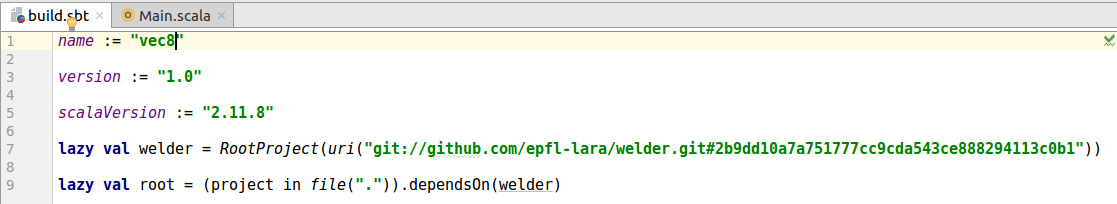
\includegraphics[scale=0.4]{./images/capt4.png}
}
\end{figure}

Next, we go to File $\to$ Settings $\to$ Build,Execution,Deployment $\to$ Build Tools $\to$ SBT and mark the option \textit{Use SBT shell for build and import (requires sbt 0.13.5+)} and press OK.

\begin{figure}[H]
\centering
\makebox[\textwidth][c]{
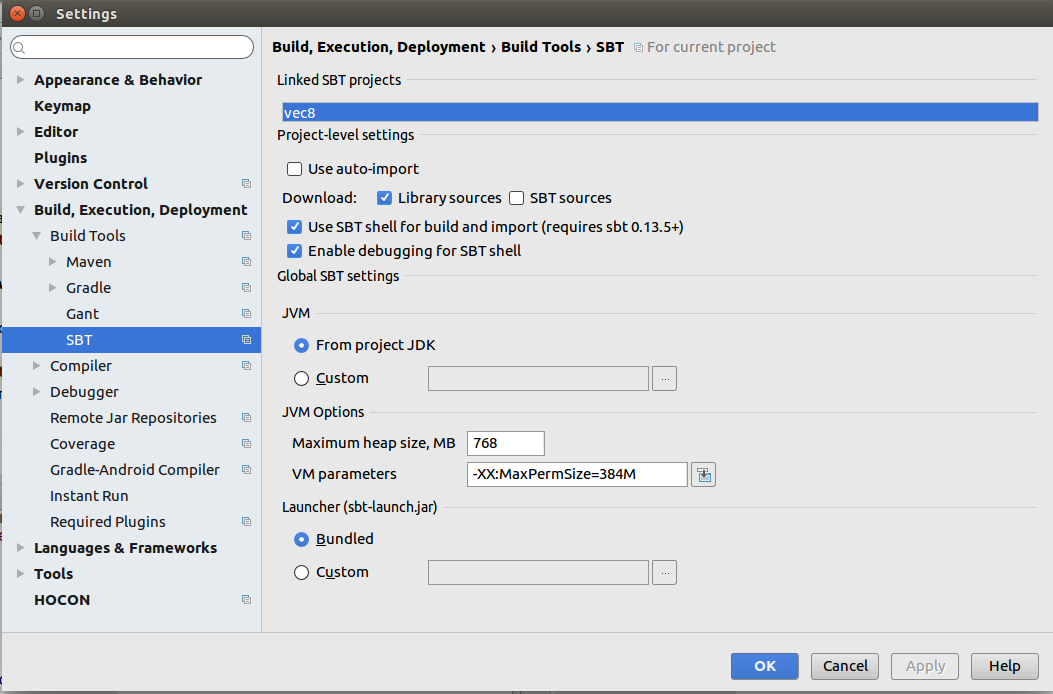
\includegraphics[scale=0.3]{./images/capt1.png}
}
\end{figure}

Finally, we select the option Refresh project that should have appeared after updating the build.sbt file. We accept, without unmarking the removal of the modules that Intellij Idea suggests. 

Once we are done, we obtain in the Project Panel three projects modules. Observe that the RootProject command in the build.sbt is highlighted. We can get rid of this by renaming the projects and build files to the following:

\begin{enumerate}
\item inox-root and inox-root-build
\item myproject-root and myproject-root-build
\item welder-root and welder-root-build
\end{enumerate}

To do so right click and the modules and then Refactor $\to$ Rename $\to$ Rename Module. Before building our project, we mark the src file in our project as source file in File $\to$ Project-Structure $\to$ Project name $\to$ Sources $\to$ src and selecting Sources icon. Then we put our Main.scala file in the corresponding directory. 

\begin{figure}[H]
\centering
\makebox[\textwidth][c]{
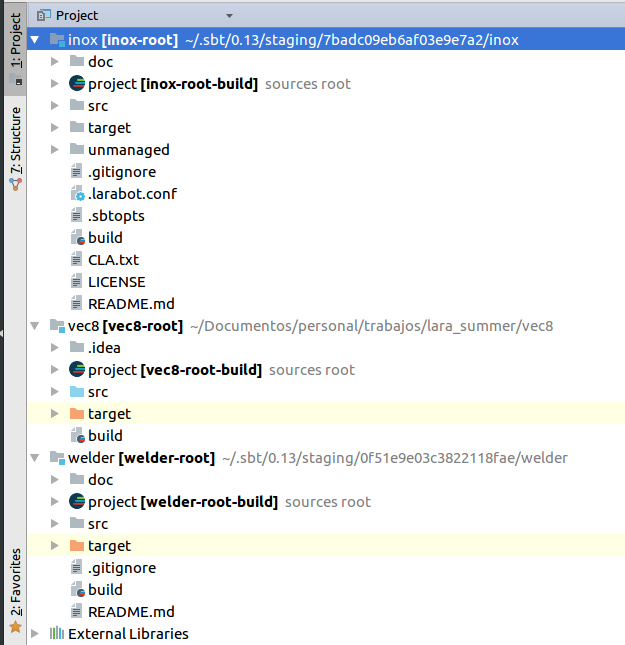
\includegraphics[scale=0.3]{./images/capt2.png}
}
\end{figure}

We also need to tell Intellij Idea that our project depends on Inox. We do so in File $\to$ Project-Structure $\to$ Project name $\to$ + $\to$ Module dependency... $\to$ inox-root.

\begin{figure}[H]
\centering
\makebox[\textwidth][c]{
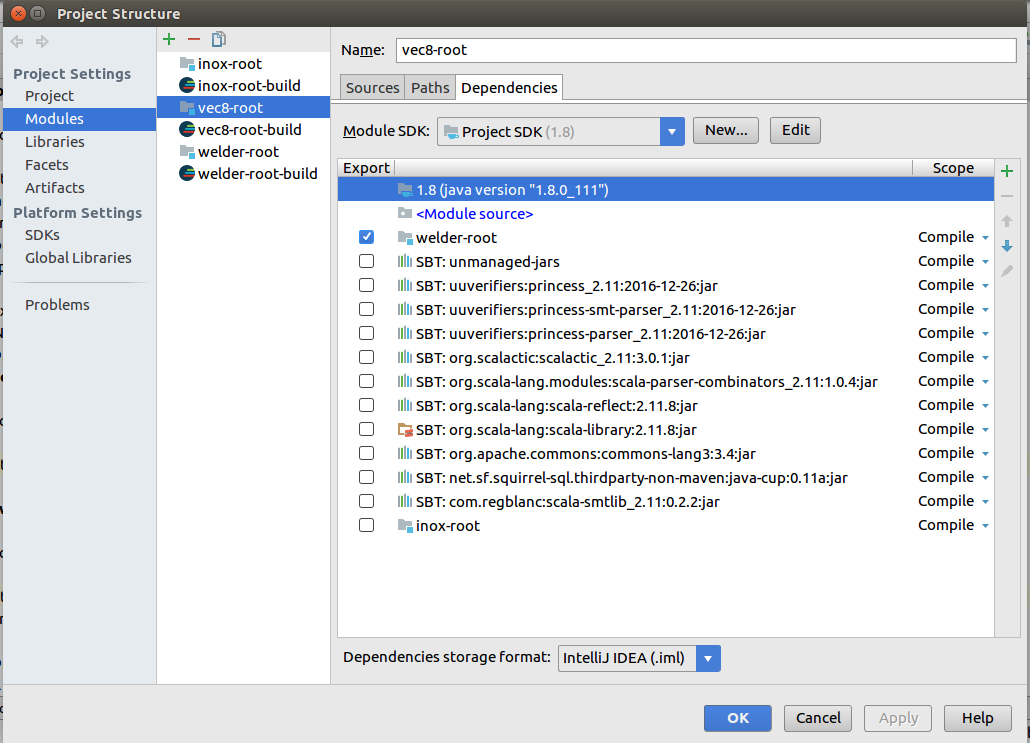
\includegraphics[scale=0.3]{./images/capt3.png}
}
\end{figure}

We set the running configuration in Run $\to$ Edit configuration $\to$ Application mode and selecting the module and the main program as usual. Before running this, we go to the SBT shell and compile the program. Finally, we run the Application as usual in Intellij Idea. 

The above configuration process can be found in references \cite{ref1}-\cite{ref7}.